\documentclass[12pt,a4paper]{article}
\usepackage{enumerate} 	% put in numbers or bullet points
\usepackage{setspace}	% line spacing					
\usepackage{authblk}	% For author affiliations
\usepackage{graphicx} 	% For adding pictures
\usepackage{pdflscape}	% for landscape pages
\usepackage{mathtools}	% For equations etc.
\usepackage[osf]{mathpazo} 
\usepackage{float}		
\floatstyle{plaintop} 	% Force table captions to go above the table
\usepackage{longtable}
\usepackage[margin ={2cm, 2cm, 2cm, 2cm}]{geometry}
\usepackage[round]{natbib}
%\setcounter{secnumdepth}{0} % removes numbers from section headings
\raggedright 			% justify the text on the left only
\pagenumbering{arabic}

	

\begin{document}

\title{
       Cranial morphological disparity within the adaptive radiation of tenrecs (Afrosoricida, Tenrecidae) is no greater than expected by chance\\
       \bigskip
       Supplementary Material }
\author{Sive Finlay and Natalie Cooper}
\date{}
\maketitle

\linespread{1.6}


%----------------------------------------------------
%Camera protocol
%---------------------------------------------------

\section{Photographing specimens}
One of us (SF) photographed the specimens with a Canon EOS 650D camera fitted with an EF 100mm f/2.8 Macro USM lens.We used a remote control (h\"ahnel Combi TF) to take the photos to avoid shaking the camera and distorting the images

We used photographic copy stands consisting of a camera attachment with an adjustable height bar, a flat stage on which to place the specimen and an adjustable light source to either side of the stage. We used the copy stands that were available at each museum which differed in how the camera height was adjusted and in the light sources available.
To take the light variability into account, on each day we took a picture of a white sheet of paper and used the custom white balance function on the camera to set the image as the baseline “white” measurement for those particular light conditions.

We photographed the specimens on a black material background with the light source in the top left-hand corner of the picture. We positioned a piece of white card on the bottom right side of the specimen to reflect the light back onto the specimen and therefore minimise any shadows (figure \ref{fig:camera} below).

%Camera picture
\begin{figure}[H] 
  \centering
  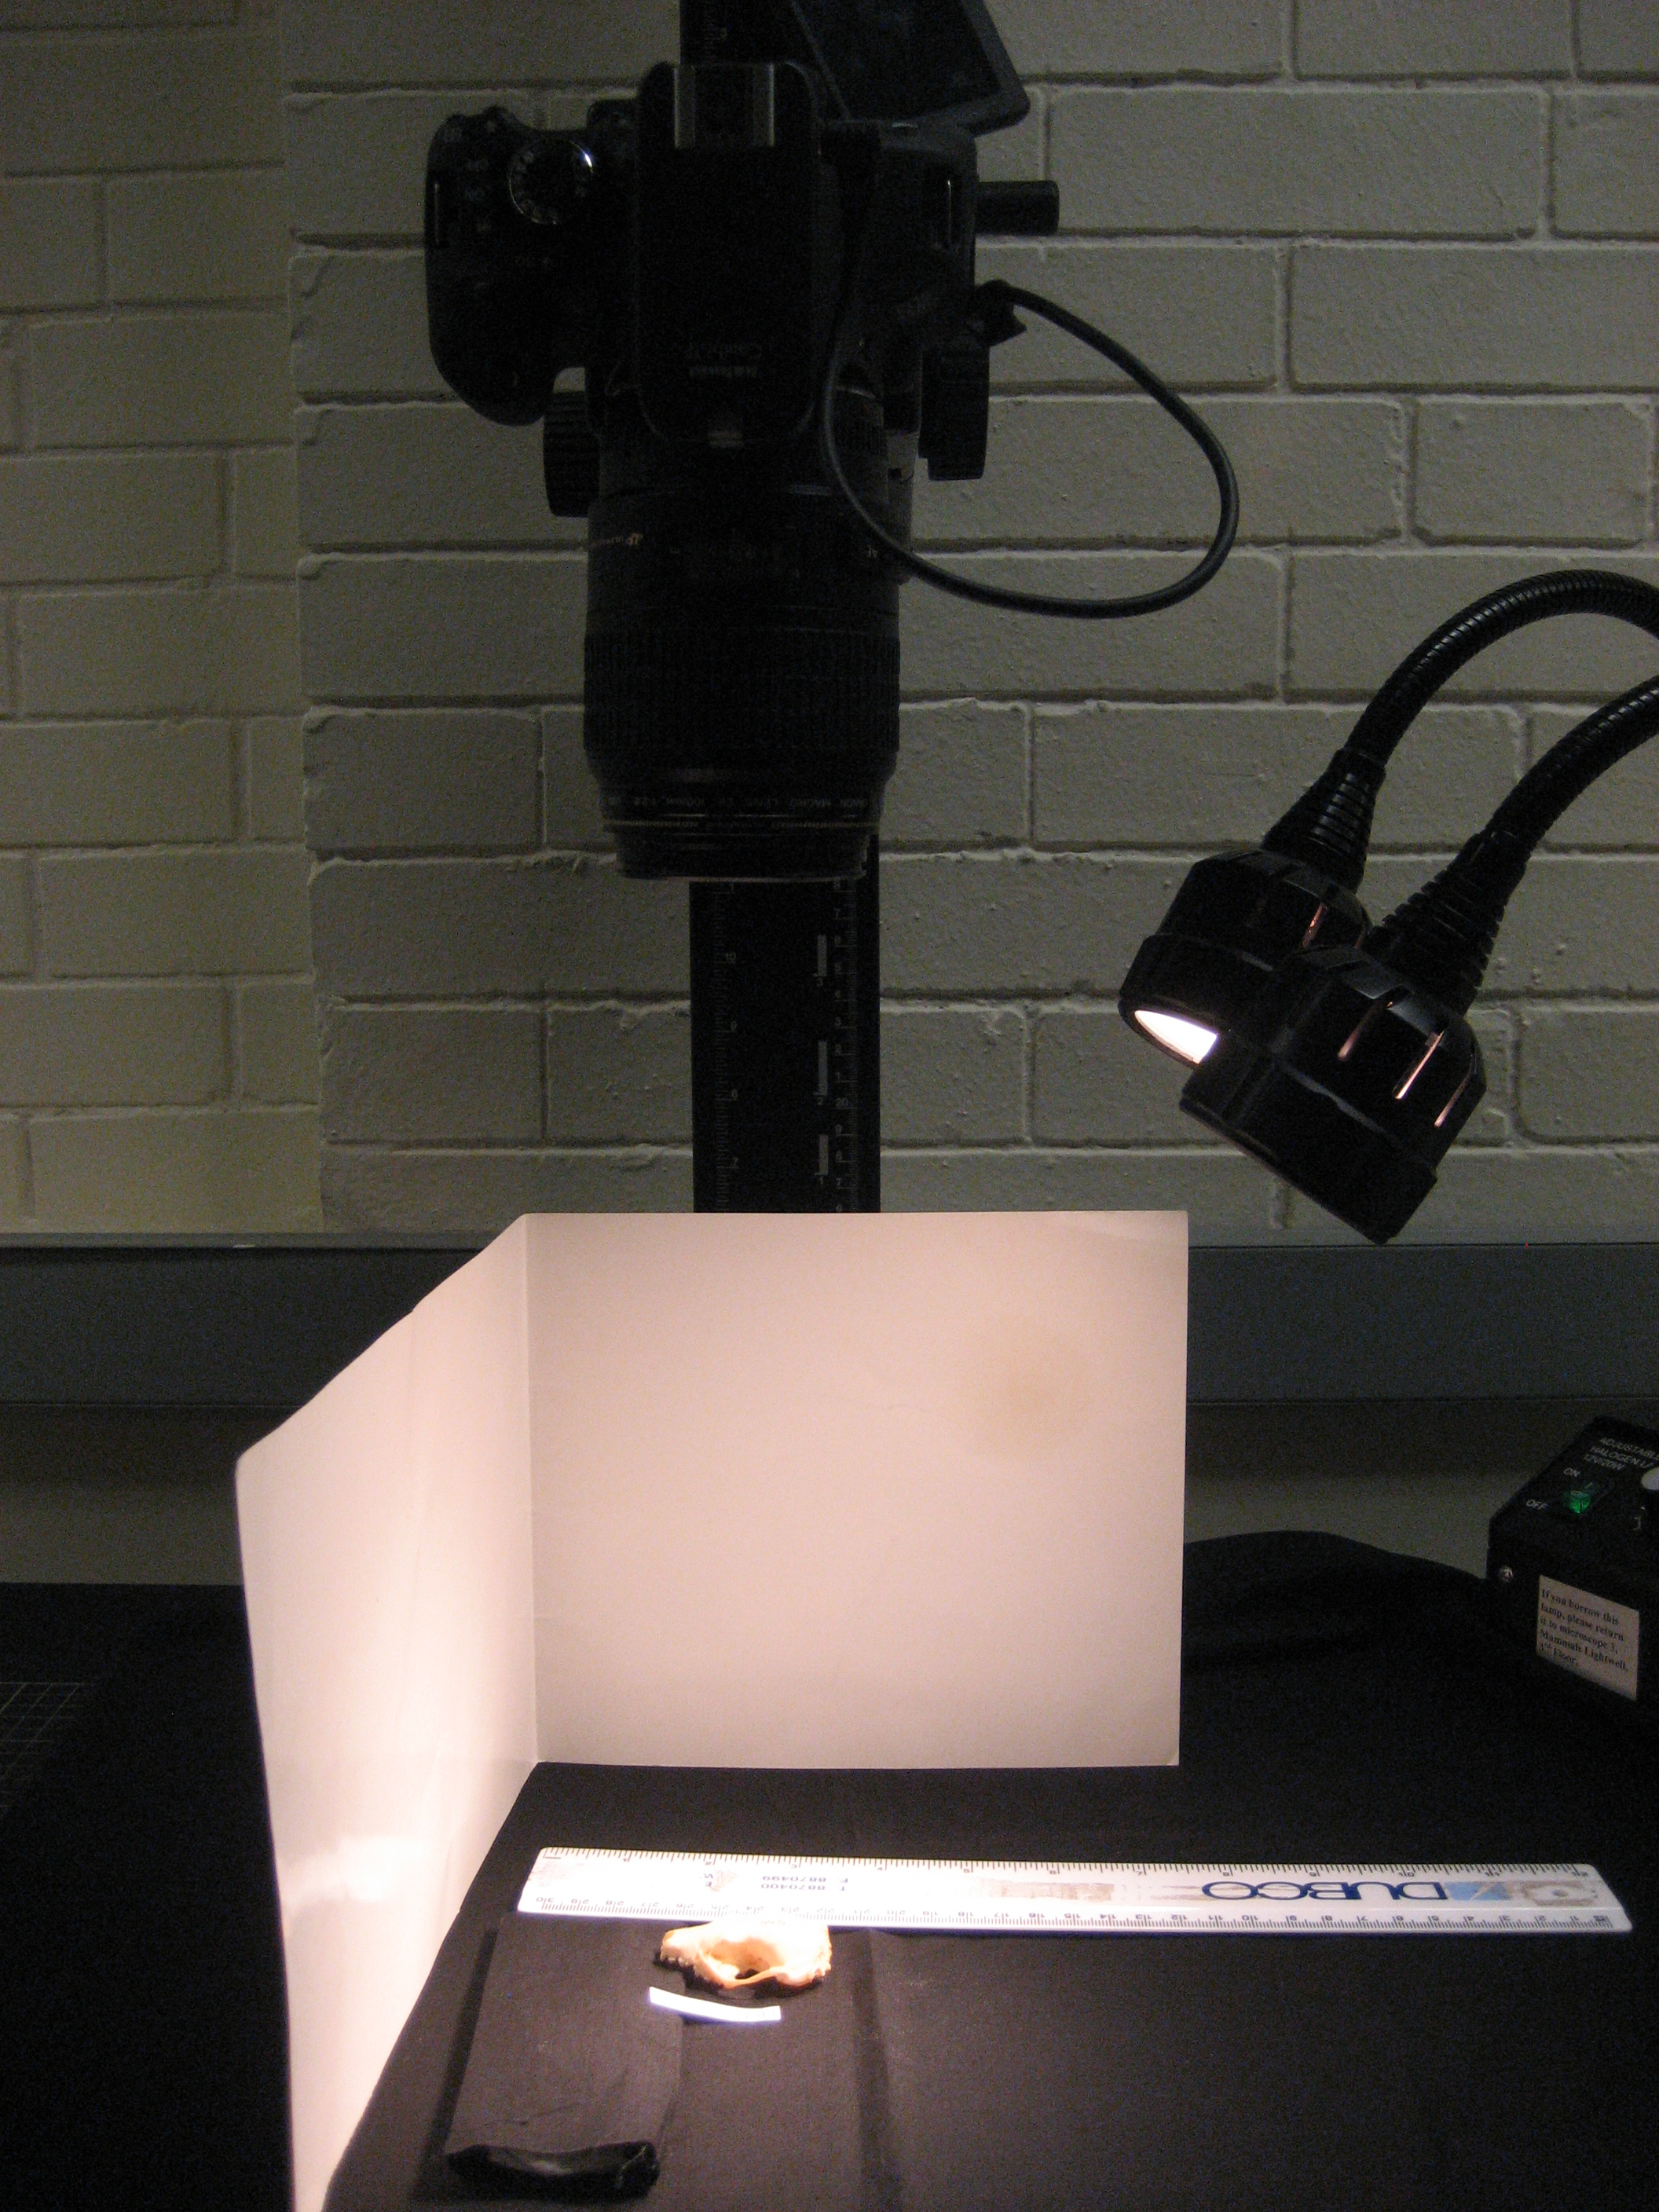
\includegraphics[width=12cm, height=12cm, keepaspectratio=true]{figures/camera.jpg}
    \caption[Photographic set up]%this is what appears in table of contents
    {Photographic set up for taking pictures of skulls. The camera (above centre) is fitted to a copy stand, the light source is directed from the top-left corner of the image and the white card reflects the light back onto the skull. }%this is under the figure
  \label{fig:camera}
  \end{figure}

%----------------------------------------------
%Resampling for minimum number of points
%-----------------------------------------
\section{Determining the number of landmarks to use for curves}
When combining landmark and semi-landmark approaches, there is a potential problem of over-sampling the curves (REFS). To determine the number of semilandmark points required to adequately summarise the curves in our data sets,  we followed the method outlined by MacLeod \citeyearpar{MacLeod2012}. 
For each data set we chose a random selection of pictures of specimens which represented the breadth of the morphological data (i.e. specimens from each sub-group of species).  We drew the appropriate curves on the each specimen and over-sampled the number of points on the curves (i.e. resampled the curves so that points were very close together). 
We measured the length of the line and regarded that as the 100\%, true length of that outline. We then re-sampled the curves with decreasing numbers of points and measured the length of the outlines. We calculated the length of the curves resampled with fewere points as a percentage of the total length of the curve. We repeated these calculations for each specimen and then found the average percentage length for each resampled curve across all of the specimens in the test file. We continued this process until we found the minimum number of points that, on average, gave a curve length which was at least a 96\% accurate representatio of the true (over-sampled) curve length.  
We repeated these curve-sampling tests for each analysis (skulls in dorsal/ventral/lateral views and mandibles in lateral view) to determine the minimum number of semilandmark points which would give accurate representations of morphological shape.

%---------------------------------------------------------
%Landmarks and results for ventral and lateral skull views
%---------------------------------------------------------
\section{Analyses of ventral and lateral skull views}

%--------------------------------------
%Sklat diagram and landmarks description
\begin{figure}[H] 
  \centering
  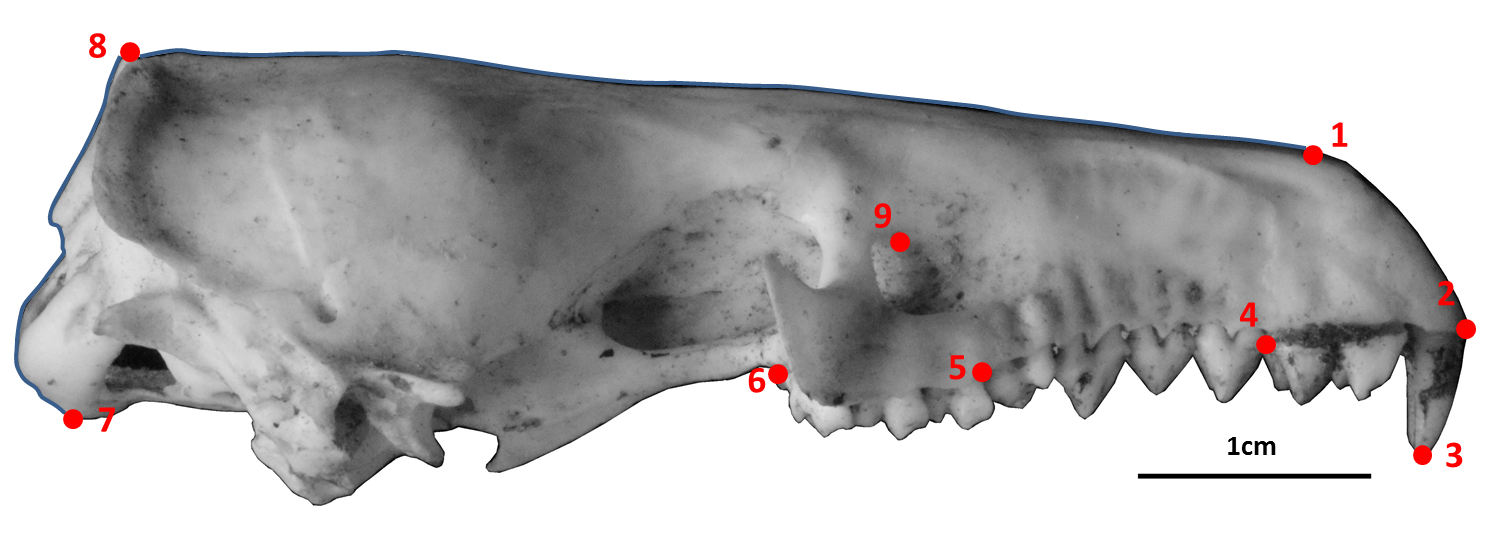
\includegraphics[width=12cm, height=12cm, keepaspectratio=true]
  {figures/sklat_landmarks_pot_vel.png}
    \caption {Landmarks (red) and curve (blue) for the ventral skull pictures, further descriptions in table \ref{tab:sklat}. The specimen is a giant otter shrew tenrec, \textit{Potamogale velox}, NHML 1934.6.16.2}
  \label{fig:sklat_landmarks}
  \end{figure}


% Skulls ventral landmarks
\begin{table}[h]
\caption{Descriptions of the landmarks (points) and curves (semilandmarks) for the skulls in ventral view (see Figure \ref{fig:sklat_landmarks}.} 
%Sklat landmarks
\begin{tabular}[t]{l l}		
\hline
\textbf{Landmark} & \textbf{Description} \\
\hline
%--------------------------------------
1 & Anterior, upper tip of the nasal bone\\
%--------------------------------------
2 & Anterior of the alveolus of the first incisor\\
%--------------------------------------
3 & Lowest point of the first incisor\\
%--------------------------------------
4& Posterior of the alveolus of the last incisor \\
%--------------------------------------
5 & Anterior tip of the alveolus of the first molar\\
%--------------------------------------
6 & Posterior tip of the alveolus of the last molar\\
%--------------------------------------
7 & Lowest point of the basi-occipital (base of the back of the skull)\\
%--------------------------------------
8 & Highest point of the braincase\\
%--------------------------------------
9 & Highest point of the infraorbital foramen\\
%--------------------------------------
\hline
\textbf{Curve A} & Between points 7 and 8  \\
(20 points)& Back of the skull from the lowest to highest points\\
%------------------------------------------------------------
\textbf{Curve B} & Between points 8 and 1  \\
(15 points)&From the highest point of the braincase to the front of the nasal \\
%------------------------------------------------------------
\hline
\end{tabular}
\label{tab:sklat}
\end{table}


%--------------------------------------
%Skvent diagram and landmarks description
\begin{figure}[H] 
  \centering
  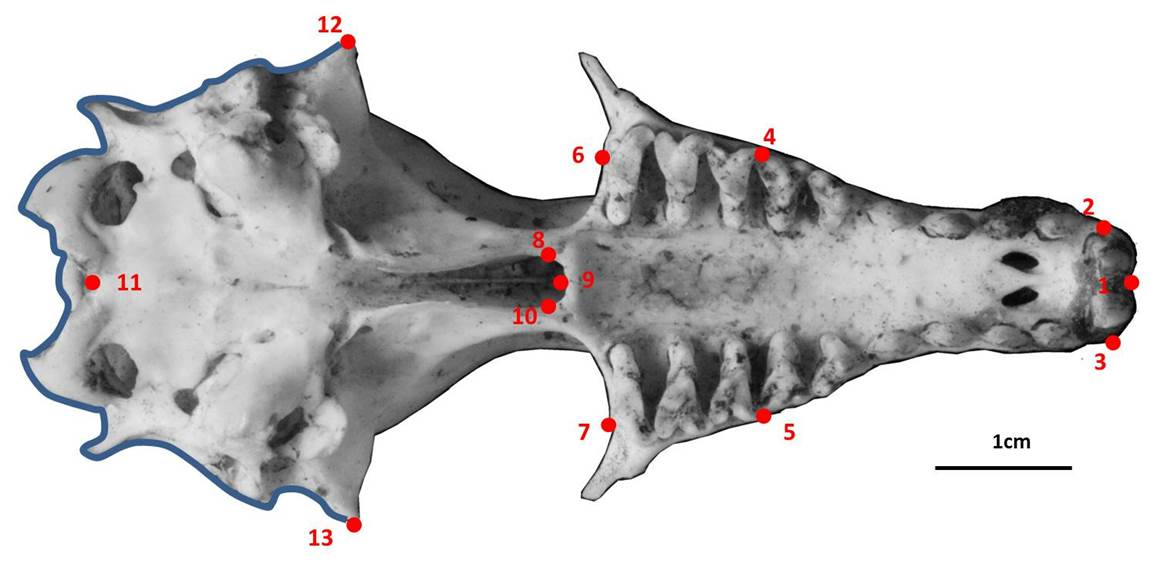
\includegraphics[width=12cm, height=12cm, keepaspectratio=true]
  {figures/skvent_landmarks_pot_vel.jpg}
    \caption {Landmarks (red) and curve (blue) for the ventral skull pictures, further descriptions in table \ref{tab:skvent}. The specimen is a giant otter shrew tenrec, \textit{Potamogale velox}, NHML 1934.6.16.2}
  \label{fig:skvent_landmarks}
  \end{figure}


% Skulls ventral landmarks
\begin{table}[h]
\caption{Descriptions of the landmarks (points) and curves (semilandmarks) for the skulls in ventral view (see Figure \ref{fig:skvent_landmarks}.} 
%SkVent landmarks
\begin{tabular}[t]{l l}		
\hline
\textbf{Landmark} & \textbf{Description} \\
\hline
%--------------------------------------
1 & Anterior point of the palate\\
%--------------------------------------
2 + 3 & Posterior, lateral extremity of the right (2) and left(3) incisor\\
%--------------------------------------
4 + 5 & Anterior, outer point of the first molar on the right (4) and left (5)\\
%--------------------------------------
6 + 7 & Posterior, outermost point of the molar surface on the right (6) and left (7) \\
%--------------------------------------
8 & Widest point of the curve of the palatine on the right side\\
%--------------------------------------
9 & Posterior point of the palatine in the midline\\
%--------------------------------------
10 & Widest point of the curve of the palatine on the left side\\
%--------------------------------------
11 & Anterior of the occipital foramen in the midline\\
%--------------------------------------
12 + 13 & Widest (extreme lateral) point of the braincase on the right (12) and left (13)\\
%--------------------------------------
Curve* & Outline of the back of the skull (between landmarks 12 and 13), 60 points \\
%------------------------------------------------------------
\hline
&*NB: This curve doesn't necessarily trace homologous features because of the \\ 
& variation in the position of the foramen magnum.
\end{tabular}
\label{tab:skvent}
\end{table}
%---------------------------------------------------------
%Rarefaction methods and results
%---------------------------------------------------------
\section{Sensitivity analyses: sample size}
Our calculations of disparity in tenrecs and golden moles are based on the amount of morphospace which is occupied by each group; families which occupy larger areas of morphospace are considered to have higher morphological disparity. However, larger groups might be expected to occupy greater areas of morphospace just because they are represented by more species. We compared a sample of 31 species of tenrec to 12 species of golden moles. Therefore, we used rarefaction analyses to test whether differences in morphospace occupation between the two groups were merely artefacts of variation in sample size.

For each data set (skulls dorsal/ventral/lateral and mandibles) we re-sampled the shape data (average shape for each species) without replacement and repeated the resampling 100 times for each iteration. For tenrecs and golden moles we re-sampled from two to n-1 species i.e. 100 samples of 2 species, 3 species, 4 species etc. We calculated disparity metrics (sum and product of variance and ranges) for each re-sampled iteration and took the average calculated value for that metric and iteration (e.g. average sum of variance from 100 sets of 2 re-sampled species). We used bootstapping (1000 iterations) to calculate 95\% confidence intervals for each sample size. We plotted the mean values and confidence intervals against sample size to depict the expected change in disparity. 

Separate discussion of each data set

%****************************************
%NB: I need to re-create these rarefaction pictures to make them nicer; the confidence intervals are too fuzzy
\begin{figure}[H] 
  \centering
  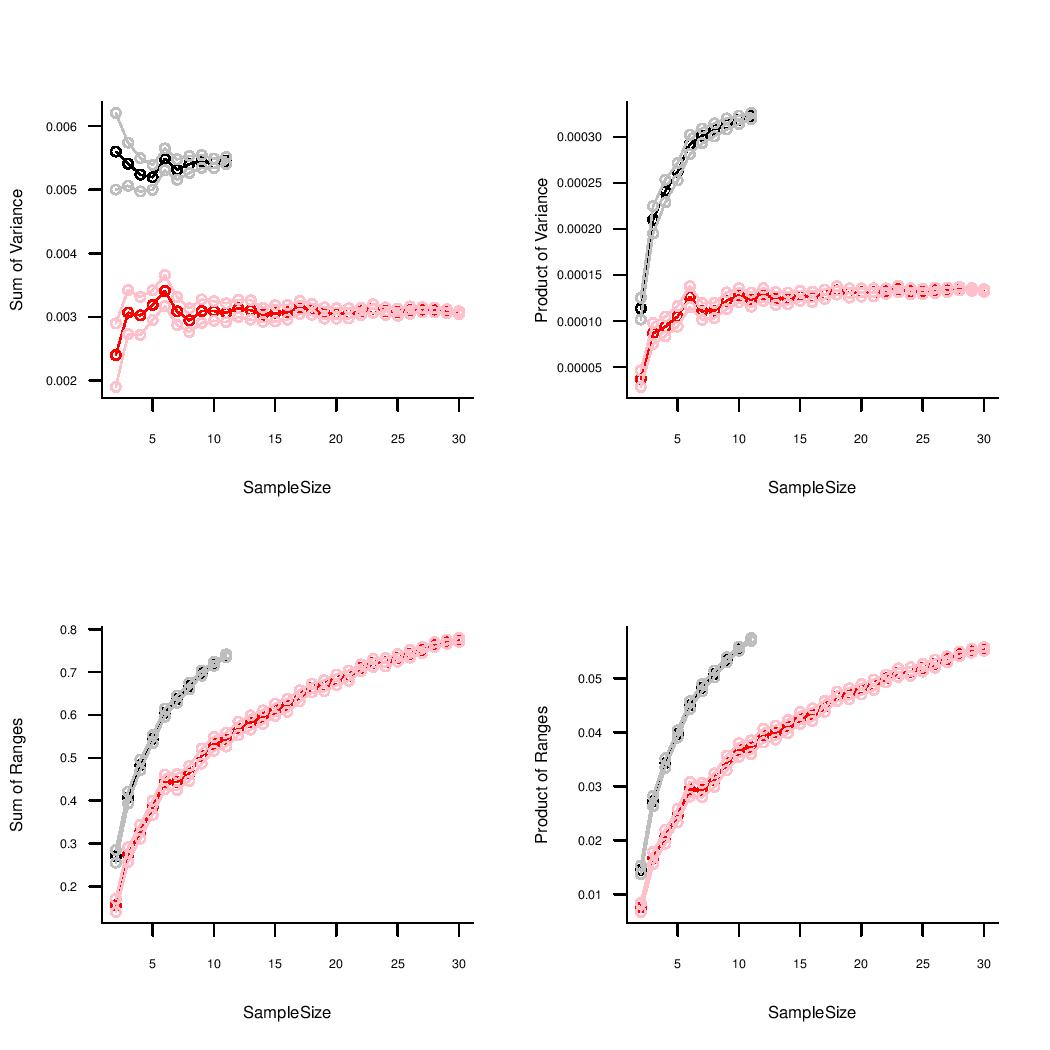
\includegraphics{figures/mands_trc+gmole_PCrarefaction.jpg}
    \caption
    {Rarefaction profiles of disparity metrics for mandibles}%this is under the figure
  \label{fig:mands.rarefaction}
  \end{figure}
%*********************************************     
%---------------------------------------------------------
%Simulation results for non-Microgale tenrecs
%---------------------------------------------------------
\section{Sensitivity analyses: comparison of non-\textit{Microgale} tenrecs}


%---------------------------------------------------------
%Table of museum accession numbers
%---------------------------------------------------------
\section{Museum specimens}
%I need to fix the position of the caption
% Table generated by Excel2LaTeX from sheet 'Tenrec_Gmole_skulls_taxonomy'

%\documentclass[12pt]{article}
%\usepackage{longtable}
%\usepackage[margin ={1cm, 1cm, 1cm, 1cm, 1cm}]{geometry}
%\pagenumbering{}
%\begin{document}

%\begin{centre}
\begin{longtable}{|l|l|l|l|l|}

  \caption{Museum accession numbers and taxonomic identification for all skull specimens. AMNH (American Museum of Natural History), FMNH (Field Museum of Natural History), MCZ (Museum of Comparative Zoology, Harvard), NHML (Natural History Museum London), SI (Smithsonian Institute)}{l}\\
  \hline 

\textbf{Specimen ID} & \textbf{Order} & \textbf{Family} & \textbf{Genus} & \textbf{Species} \\
\hline
\endfirsthead

\multicolumn {5} {l}
{{\bfseries \tablename\ \thetable\ --\textit{Continues from previous page}}}\\
  \hline
  \textbf{SpecID} & \textbf{Order} & \textbf{Family} & \textbf{Genus} & \textbf{Species} \\
  \hline
\endhead

\hline \multicolumn{5}{|r|}{\textit{Continued on next page}} \\ 
\hline
\endfoot


\hline 
\endlastfoot

    AMNH\_161526 & Afrosoricida & Chrysochloridae & Chlorotalpa & duthieae \\
    AMNH\_161527 & Afrosoricida & Chrysochloridae & Chlorotalpa & duthieae \\
    AMNH\_161559 & Afrosoricida & Chrysochloridae & Eremitalpa & granti \\
    AMNH\_161571 & Afrosoricida & Chrysochloridae & Eremitalpa & granti \\
    AMNH\_167961 & Afrosoricida & Chrysochloridae & Chrysochloris & asiatica \\
    AMNH\_180911 & Afrosoricida & Chrysochloridae & Chrysochloris & stuhlmanni \\
    AMNH\_180912 & Afrosoricida & Chrysochloridae & Chrysochloris & stuhlmanni \\
    AMNH\_212938 & Afrosoricida & Tenrecidae & Hemicentetes & semispinosus \\
    AMNH\_274982 & Afrosoricida & Tenrecidae & Microgale & jobihely \\
    AMNH\_274986 & Afrosoricida & Tenrecidae & Microgale & jobihely \\
    AMNH\_274987 & Afrosoricida & Tenrecidae & Microgale & jobihely \\
    AMNH\_274988 & Afrosoricida & Tenrecidae & Microgale & jobihely \\
    AMNH\_274989 & Afrosoricida & Tenrecidae & Microgale & jobihely \\
    AMNH\_275041 & Afrosoricida & Tenrecidae & Microgale & soricoides \\
    AMNH\_275088 & Afrosoricida & Tenrecidae & Microgale & drouhardi \\
    AMNH\_275089 & Afrosoricida & Tenrecidae & Microgale & drouhardi \\
    AMNH\_275090 & Afrosoricida & Tenrecidae & Microgale & drouhardi \\
    AMNH\_275092 & Afrosoricida & Tenrecidae & Microgale & drouhardi \\
    AMNH\_275095 & Afrosoricida & Tenrecidae & Microgale & drouhardi \\
    AMNH\_275133 & Afrosoricida & Tenrecidae & Microgale & fotsifotsy \\
    AMNH\_275134 & Afrosoricida & Tenrecidae & Microgale & gymnorhyncha \\
    AMNH\_275135 & Afrosoricida & Tenrecidae & Microgale & gymnorhyncha \\
    AMNH\_275136 & Afrosoricida & Tenrecidae & Microgale & gymnorhyncha \\
    AMNH\_275137 & Afrosoricida & Tenrecidae & Microgale & gymnorhyncha \\
    AMNH\_275138 & Afrosoricida & Tenrecidae & Microgale & gymnorhyncha \\
    AMNH\_275141 & Afrosoricida & Tenrecidae & Microgale & longicaudata \\
    AMNH\_275142 & Afrosoricida & Tenrecidae & Microgale & longicaudata \\
    AMNH\_275143 & Afrosoricida & Tenrecidae & Microgale & longicaudata \\
    AMNH\_275148 & Afrosoricida & Tenrecidae & Microgale & longicaudata \\
    AMNH\_275149 & Afrosoricida & Tenrecidae & Microgale & longicaudata \\
    AMNH\_275157 & Afrosoricida & Tenrecidae & Microgale & parvula \\
    AMNH\_275158 & Afrosoricida & Tenrecidae & Microgale & soricoides \\
    AMNH\_275160 & Afrosoricida & Tenrecidae & Microgale & soricoides \\
    AMNH\_275162 & Afrosoricida & Tenrecidae & Microgale & soricoides \\
    AMNH\_275163 & Afrosoricida & Tenrecidae & Microgale & soricoides \\
    AMNH\_275189 & Afrosoricida & Tenrecidae & Oryzorictes & hova \\
    AMNH\_275190 & Afrosoricida & Tenrecidae & Oryzorictes & hova \\
    AMNH\_275191 & Afrosoricida & Tenrecidae & Oryzorictes & hova \\
    AMNH\_275250 & Afrosoricida & Tenrecidae & Microgale & brevicaudata \\
    AMNH\_275251 & Afrosoricida & Tenrecidae & Microgale & brevicaudata \\
    AMNH\_275253 & Afrosoricida & Tenrecidae & Microgale & brevicaudata \\
    AMNH\_275254 & Afrosoricida & Tenrecidae & Microgale & brevicaudata \\
    AMNH\_275255 & Afrosoricida & Tenrecidae & Microgale & brevicaudata \\
    AMNH\_275281 & Afrosoricida & Tenrecidae & Microgale & fotsifotsy \\
    AMNH\_275282 & Afrosoricida & Tenrecidae & Microgale & fotsifotsy \\
    AMNH\_275283 & Afrosoricida & Tenrecidae & Microgale & fotsifotsy \\
    AMNH\_275298 & Afrosoricida & Tenrecidae & Microgale & taiva \\
    AMNH\_275299 & Afrosoricida & Tenrecidae & Microgale & taiva \\
    AMNH\_275300 & Afrosoricida & Tenrecidae & Microgale & taiva \\
    AMNH\_275301 & Afrosoricida & Tenrecidae & Microgale & taiva \\
    AMNH\_275360 & Afrosoricida & Tenrecidae & Oryzorictes & hova \\
    AMNH\_275364 & Afrosoricida & Tenrecidae & Microgale & parvula \\
    AMNH\_275365 & Afrosoricida & Tenrecidae & Microgale & parvula \\
    AMNH\_275368 & Afrosoricida & Tenrecidae & Microgale & parvula \\
    AMNH\_31243 & Afrosoricida & Tenrecidae & Oryzorictes & tetradactylus \\
    AMNH\_31257 & Afrosoricida & Tenrecidae & Oryzorictes & tetradactylus \\
    AMNH\_31270 & Afrosoricida & Tenrecidae & Echinops & telfairi \\
    AMNH\_34647 & Afrosoricida & Chrysochloridae & Chrysospalax & trevelyani \\
    AMNH\_51324 & Afrosoricida & Tenrecidae & Potamogale & velox \\
    AMNH\_51327 & Afrosoricida & Tenrecidae & Potamogale & velox \\
    AMNH\_54365 & Afrosoricida & Chrysochloridae & Chrysospalax & trevelyani \\
    AMNH\_82399 & Afrosoricida & Chrysochloridae & Chrysochloris & stuhlmanni \\
    AMNH\_89040 & Afrosoricida & Chrysochloridae & Chrysospalax & trevelyani \\
    AMNH\_89046 & Afrosoricida & Chrysochloridae & Cryptochloris & wintoni \\
    FMNH\_156226 & Afrosoricida & Tenrecidae & Oryzorictes & tetradactylus \\
    FMNH\_159672 & Afrosoricida & Tenrecidae & Microgale & monticola \\
    FMNH\_159673 & Afrosoricida & Tenrecidae & Microgale & monticola \\
    FMNH\_159674 & Afrosoricida & Tenrecidae & Microgale & monticola \\
    FMNH\_159675 & Afrosoricida & Tenrecidae & Microgale & monticola \\
    FMNH\_159676 & Afrosoricida & Tenrecidae & Microgale & monticola \\
    FMNH\_162893 & Afrosoricida & Tenrecidae & Micropotamogale & lamottei \\
    FMNH\_166040 & Afrosoricida & Tenrecidae & Microgale & pusilla \\
    FMNH\_166111 & Afrosoricida & Tenrecidae & Microgale & gracilis \\
    FMNH\_166112 & Afrosoricida & Tenrecidae & Microgale & gracilis \\
    FMNH\_166113 & Afrosoricida & Tenrecidae & Microgale & gracilis \\
    FMNH\_166145 & Afrosoricida & Tenrecidae & Microgale & gracilis \\
    FMNH\_167427 & Afrosoricida & Tenrecidae & Microgale & dryas \\
    FMNH\_167621 & Afrosoricida & Tenrecidae & Microgale & pusilla \\
    FMNH\_176203 & Afrosoricida & Tenrecidae & Geogale & aurita \\
    FMNH\_176204 & Afrosoricida & Tenrecidae & Geogale & aurita \\
    FMNH\_176211 & Afrosoricida & Tenrecidae & Geogale & aurita \\
    FMNH\_176385 & Afrosoricida & Tenrecidae & Microgale & dryas \\
    FMNH\_176387 & Afrosoricida & Tenrecidae & Microgale & dryas \\
    FMNH\_176389 & Afrosoricida & Tenrecidae & Microgale & dryas \\
    FMNH\_176395 & Afrosoricida & Tenrecidae & Microgale & dryas \\
    FMNH\_209199 & Afrosoricida & Tenrecidae & Microgale & grandidieri \\
    FMNH\_209200 & Afrosoricida & Tenrecidae & Microgale & grandidieri \\
    FMNH\_209201 & Afrosoricida & Tenrecidae & Microgale & grandidieri \\
    FMNH\_209202 & Afrosoricida & Tenrecidae & Microgale & grandidieri \\
    FMNH\_209203 & Afrosoricida & Tenrecidae & Microgale & grandidieri \\
    FMNH\_53073 & Afrosoricida & Chrysochloridae & Amblysomus & corriae \\
    FMNH\_72831 & Afrosoricida & Tenrecidae & Potamogale & velox \\
    FMNH\_81731 & Afrosoricida & Chrysochloridae & Calcochloris & leucorhinus \\
    FMNH\_83540 & Afrosoricida & Chrysochloridae & Calcochloris & leucorhinus \\
    MCZ\_23373 & Afrosoricida & Chrysochloridae & Chrysochloris & stuhlmanni \\
    MCZ\_45021 & Afrosoricida & Tenrecidae & Oryzorictes & tetradactylus \\
    MCZ\_45022 & Afrosoricida & Tenrecidae & Oryzorictes & tetradactylus \\
    MCZ\_45033 & Afrosoricida & Tenrecidae & Microgale & pusilla \\
    MCZ\_45050 & Afrosoricida & Tenrecidae & Limnogale & mergulus \\
    MCZ\_45450 & Afrosoricida & Tenrecidae & Geogale & aurita \\
    MCZ\_46274 & Afrosoricida & Tenrecidae & Geogale & aurita \\
    NHML\_1870.3.10.15\_1527.a & Afrosoricida & Tenrecidae & Setifer & setosus \\
    NHML\_1934.6.16.2 & Afrosoricida & Tenrecidae & Potamogale & velox \\
    NHML\_1961.6.2.3 & Afrosoricida & Chrysochloridae & Chrysospalax & trevelyani \\
    NHML\_3.1.1.1 & Afrosoricida & Tenrecidae & Geogale & aurita \\
    NHML\_3.6.2.10 & Afrosoricida & Chrysochloridae & Amblysomus & hottentotus \\
    NHML\_3509 & Afrosoricida & Tenrecidae & Tenrec & ecaudatus \\
    NHML\_67.213 & Afrosoricida & Tenrecidae & Micropotamogale & ruwenzorii \\
    NHML\_73.170 & Afrosoricida & Tenrecidae & Micropotamogale & lamottei \\
    NHML\_74.668 & Afrosoricida & Chrysochloridae & Chrysochloris & sp. \\
    NHML\_75.2223 & Afrosoricida & Tenrecidae & Microgale & cowani \\
    NHML\_82.3.1.11 & Afrosoricida & Tenrecidae & Hemicentetes & nigriceps \\
    SI\_083658 & Afrosoricida & Tenrecidae & Hemicentetes & semispinosus \\
    SI\_154988 & Afrosoricida & Tenrecidae & Microgale & dobsoni \\
    SI\_154989 & Afrosoricida & Tenrecidae & Oryzorictes & tetradactylus \\
    SI\_221420 & Afrosoricida & Chrysochloridae & Chlorotalpa & duthieae \\
    SI\_266897 & Afrosoricida & Tenrecidae & Potamogale & velox \\
    SI\_294497 & Afrosoricida & Tenrecidae & Setifer & setosus \\
    SI\_294504 & Afrosoricida & Tenrecidae & Hemicentetes & semispinosus \\
    SI\_294507 & Afrosoricida & Tenrecidae & Hemicentetes & nigriceps \\
    SI\_294508 & Afrosoricida & Tenrecidae & Hemicentetes & nigriceps \\
    SI\_294510 & Afrosoricida & Tenrecidae & Hemicentetes & nigriceps \\
    SI\_294511 & Afrosoricida & Tenrecidae & Hemicentetes & nigriceps \\
    SI\_294520 & Afrosoricida & Tenrecidae & Microgale & dobsoni \\
    SI\_328604 & Afrosoricida & Tenrecidae & Setifer & setosus \\
    SI\_328605 & Afrosoricida & Tenrecidae & Setifer & setosus \\
    SI\_328614 & Afrosoricida & Tenrecidae & Setifer & setosus \\
    SI\_328616 & Afrosoricida & Tenrecidae & Echinops & telfairi \\
    SI\_328619 & Afrosoricida & Tenrecidae & Echinops & telfairi \\
    SI\_328622 & Afrosoricida & Tenrecidae & Echinops & telfairi \\
    SI\_328624 & Afrosoricida & Tenrecidae & Echinops & telfairi \\
    SI\_328653 & Afrosoricida & Tenrecidae & Microgale & cowani \\
    SI\_328662 & Afrosoricida & Tenrecidae & Microgale & cowani \\
    SI\_328667 & Afrosoricida & Tenrecidae & Microgale & cowani \\
    SI\_328669 & Afrosoricida & Tenrecidae & Microgale & cowani \\
    SI\_328670 & Afrosoricida & Tenrecidae & Microgale & cowani \\
    SI\_328688 & Afrosoricida & Tenrecidae & Microgale & pusilla \\
    SI\_328689 & Afrosoricida & Tenrecidae & Microgale & pusilla \\
    SI\_328690 & Afrosoricida & Tenrecidae & Microgale & pusilla \\
    SI\_328695 & Afrosoricida & Tenrecidae & Microgale & dobsoni \\
    SI\_341621 & Afrosoricida & Tenrecidae & Tenrec & ecaudatus \\
    SI\_341624 & Afrosoricida & Tenrecidae & Tenrec & ecaudatus \\
    SI\_341661 & Afrosoricida & Tenrecidae & Hemicentetes & semispinosus \\
    SI\_341688 & Afrosoricida & Tenrecidae & Hemicentetes & semispinosus \\
    SI\_341689 & Afrosoricida & Tenrecidae & Hemicentetes & semispinosus \\
    SI\_351334 & Afrosoricida & Chrysochloridae & Calcochloris & obtusirostris \\
    SI\_351335 & Afrosoricida & Chrysochloridae & Calcochloris & obtusirostris \\
    SI\_351336 & Afrosoricida & Chrysochloridae & Chrysospalax & villosus \\
    SI\_351955 & Afrosoricida & Chrysochloridae & Calcochloris & obtusirostris \\
    SI\_361482 & Afrosoricida & Tenrecidae & Tenrec & ecaudatus \\
    SI\_365001 & Afrosoricida & Chrysochloridae & Carpitalpa & arendsi \\
    SI\_380484 & Afrosoricida & Chrysochloridae & Amblysomus & hottentotus \\
    SI\_380485 & Afrosoricida & Chrysochloridae & Amblysomus & hottentotus \\
    SI\_381488 & Afrosoricida & Chrysochloridae & Amblysomus & hottentotus \\
    SI\_395676 & Afrosoricida & Tenrecidae & Geogale & aurita \\
    SI\_449177 & Afrosoricida & Tenrecidae & Microgale & taiva \\
    SI\_449179 & Afrosoricida & Tenrecidae & Microgale & gracilis \\
    SI\_449192 & Afrosoricida & Tenrecidae & Microgale & dobsoni \\
    SI\_468315 & Afrosoricida & Chrysochloridae & Chrysochloris & asiatica \\
    SI\_468316 & Afrosoricida & Chrysochloridae & Chrysochloris & asiatica \\
    SI\_468317 & Afrosoricida & Chrysochloridae & Chrysochloris & asiatica \\
    SI\_468318 & Afrosoricida & Chrysochloridae & Eremitalpa & granti \\
    SI\_468319 & Afrosoricida & Chrysochloridae & Cryptochloris & wintoni \\
    SI\_470211 & Afrosoricida & Chrysochloridae & Calcochloris & obtusirostris \\
    SI\_537651 & Afrosoricida & Tenrecidae & Potamogale & velox \\
    SI\_577052 & Afrosoricida & Tenrecidae & Oryzorictes & hova \\
    SI\_577055 & Afrosoricida & Tenrecidae & Microgale & talazaci \\
    SI\_578746 & Afrosoricida & Tenrecidae & Microgale & talazaci \\
    SI\_578747 & Afrosoricida & Tenrecidae & Microgale & talazaci \\
    SI\_578749 & Afrosoricida & Tenrecidae & Microgale & dobsoni \\
    SI\_578753 & Afrosoricida & Tenrecidae & Microgale & principula \\
    SI\_578756 & Afrosoricida & Tenrecidae & Microgale & principula \\
    SI\_578759 & Afrosoricida & Tenrecidae & Microgale & principula \\
    SI\_578760 & Afrosoricida & Tenrecidae & Microgale & principula \\
    SI\_578762 & Afrosoricida & Tenrecidae & Microgale & principula \\
    SI\_578768 & Afrosoricida & Tenrecidae & Microgale & talazaci \\
    SI\_578769 & Afrosoricida & Tenrecidae & Microgale & talazaci \\
    SI\_578772 & Afrosoricida & Tenrecidae & Microgale & thomasi \\
    SI\_578773 & Afrosoricida & Tenrecidae & Microgale & thomasi \\
    SI\_578774 & Afrosoricida & Tenrecidae & Microgale & thomasi \\
    SI\_578775 & Afrosoricida & Tenrecidae & Microgale & thomasi \\
    SI\_578776 & Afrosoricida & Tenrecidae & Microgale & thomasi \\
    SI\_578784 & Afrosoricida & Tenrecidae & Microgale & parvula \\
    SI\_578787 & Afrosoricida & Tenrecidae & Microgale & fotsifotsy \\
    SI\_578789 & Afrosoricida & Tenrecidae & Oryzorictes & sp. \\
    SI\_578791 & Afrosoricida & Tenrecidae & Tenrec & ecaudatus \\
    SI\_578792 & Afrosoricida & Tenrecidae & Tenrec & ecaudatus \\
    SI\_584649 & Afrosoricida & Chrysochloridae & Calcochloris & leucorhinus \\

\end{longtable}
%\end{centre}
%\end{document}

%  \label{tab:sk.taxonomy}%
%\end{table}%

\bibliographystyle{jeb}
\bibliography{Refs_01_05_14_edited}
\end{document}